\documentclass[tikz,border=5pt]{standalone}
\usetikzlibrary{calc}
\usepackage{tikz}
\usetikzlibrary{arrows.meta,positioning}

\begin{document}

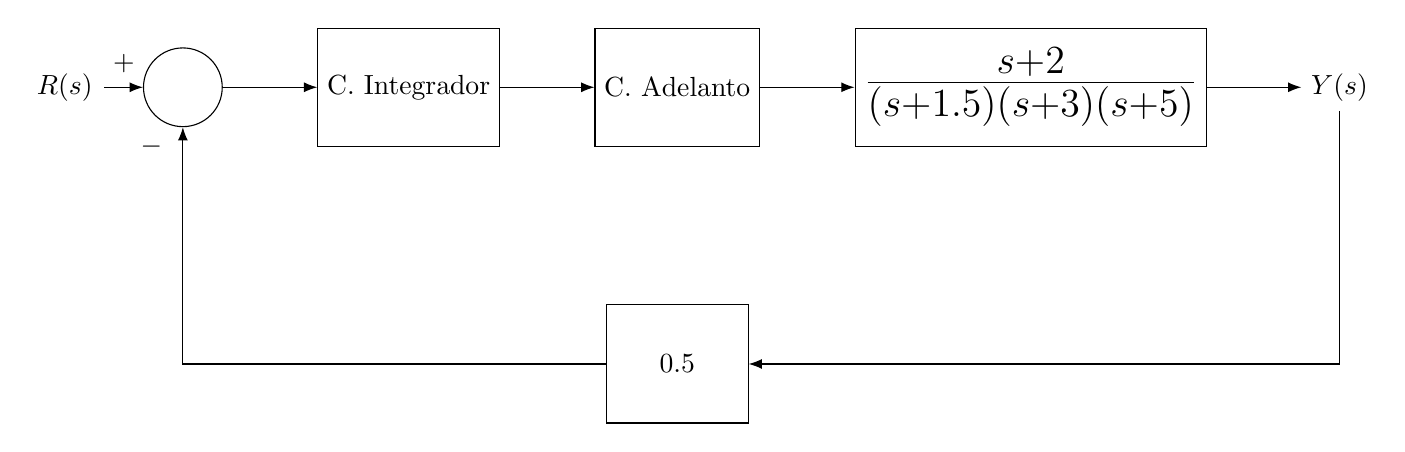
\begin{tikzpicture}[
    >=Latex,
    node distance=1.2cm,
    block/.style={draw, rectangle, minimum height=1.5cm, minimum width=1.8cm},
    sum/.style={draw, circle, minimum size=1cm}
]

% Entrada
\node at (-1.5,0) {$R(s)$};

% Sumador
\node[sum] (sum) {};

% Bloques
\node[block, right=of sum, minimum width=1.5cm] (int) {C. Integrador};

\node[block, right=of int, minimum width=1.5cm] (lead) {C. Adelanto};

\node[block, right=of lead, minimum width=3.5cm] (plant)
{\huge $\frac{s+2}{(s+1.5)(s+3)(s+5)}$};

% Salida
\node[right=of plant] (y) {$Y(s)$};

% Sensor
\node[block, below=2cm of lead] (sensor) {$0.5$};

% Conexiones
\draw[->] (-1,0) -- (sum);
\draw[->] (sum) -- (int);
\draw[->] (int) -- (lead);
\draw[->] (lead) -- (plant);
\draw[->] (plant) -- (y);

% Realimentación
\draw[->] (y) |- (sensor);
\draw[->] (sensor) -| (sum);

% Signos
\node at ($(sum)+(-0.75,0.3)$) {$+$};
\node at ($(sum)-(0.4,0.75)$) {$-$};

\end{tikzpicture}

\end{document}